\documentclass[tikz,border=5pt]{standalone}
\usepackage{amsmath}
\usetikzlibrary{arrows.meta,positioning,fit,backgrounds,shapes.geometric,calc}
\definecolor{nodec}{RGB}{225,236,246}
\definecolor{edgec}{RGB}{247,231,216}
\definecolor{fieldc}{RGB}{226,242,228}
\definecolor{opl}{RGB}{40,90,150}      % Lateral
\definecolor{opr}{RGB}{170,90,30}      % Rewire
\definecolor{opd}{RGB}{25,115,55}      % Divide / Die
\definecolor{ope}{RGB}{120,60,150}     % Exchange
\definecolor{grayt}{RGB}{95,95,95}
\definecolor{intred}{RGB}{190,55,40}
\newcommand{\code}[1]{\texttt{#1}}
\begin{document}
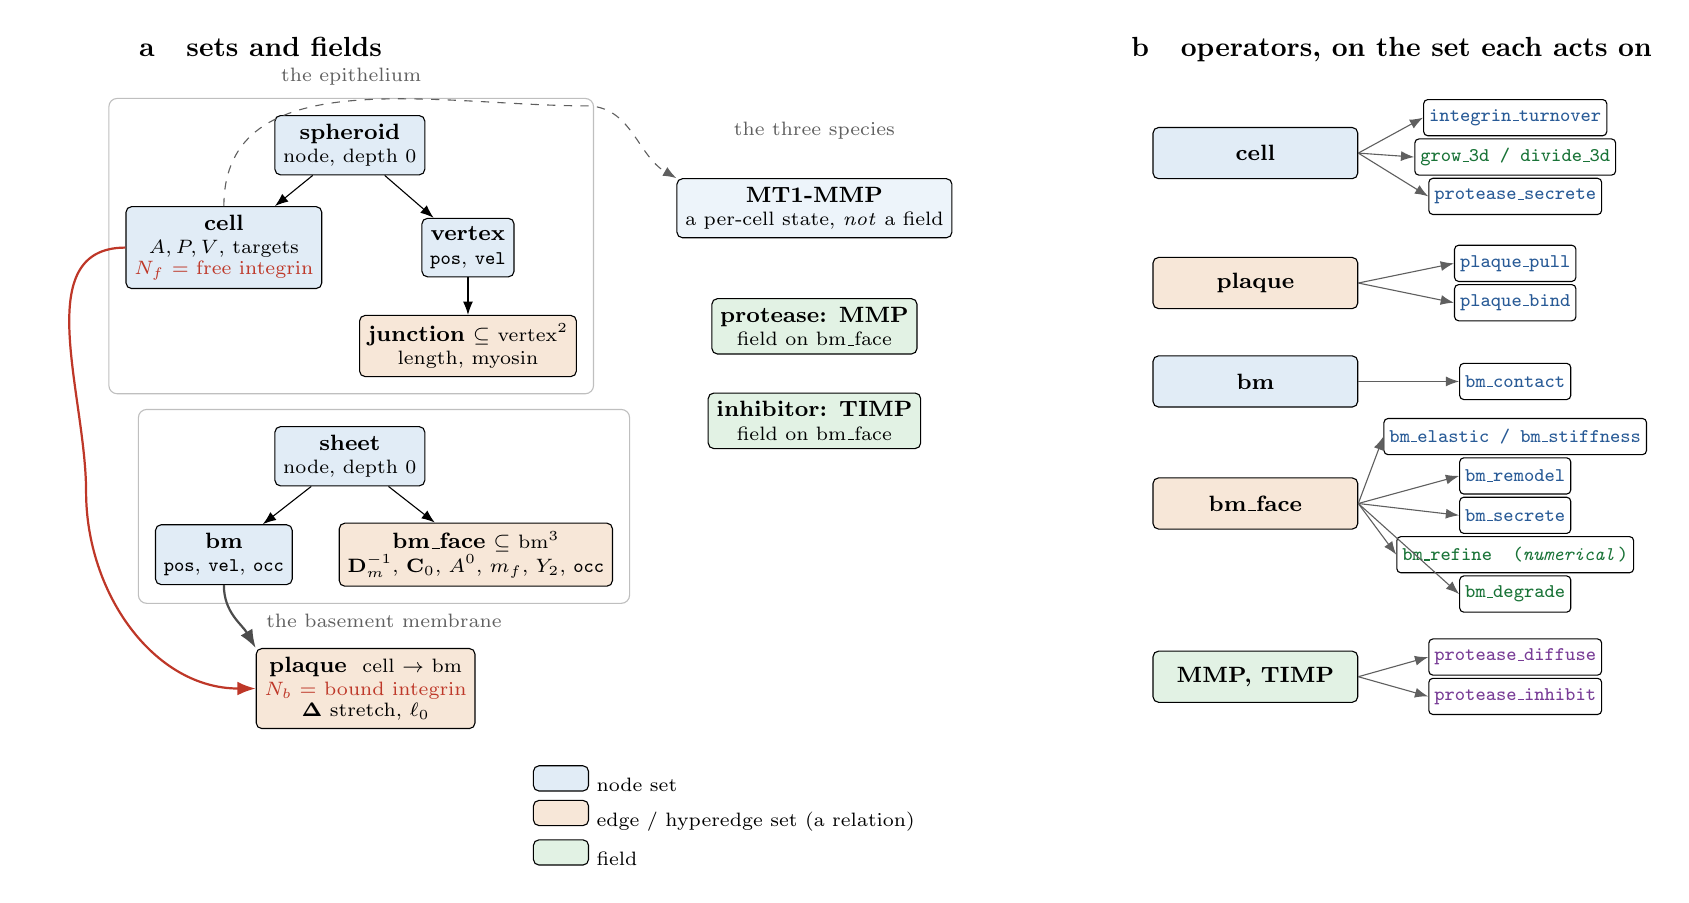
\begin{tikzpicture}[font=\footnotesize,>=Latex,
  nod/.style={draw,rounded corners=2pt,fill=nodec,minimum height=6.5mm,align=center,inner sep=3pt},
  edg/.style={draw,rounded corners=2pt,fill=edgec,minimum height=6.5mm,align=center,inner sep=3pt},
  fld/.style={draw,rounded corners=2pt,fill=fieldc,minimum height=6.5mm,align=center,inner sep=3pt},
  op/.style={draw,rounded corners=1.5pt,fill=white,minimum height=4.6mm,align=center,inner sep=2pt,
             font=\scriptsize\ttfamily}]

%============================== a: the hierarchy ==============================
\node[anchor=north west,font=\bfseries\normalsize] at (-0.4,6.9) {a\quad sets and fields};

\node[nod] (sph) at (2.4,5.4) {\textbf{spheroid}\\[-1pt]\scriptsize node, depth 0};
\node[nod] (cell) at (0.8,4.1) {\textbf{cell}\\[-1pt]
   \scriptsize $A,P,V$, targets\\[-2pt]
   \scriptsize\textcolor{intred}{$N_f$ = free integrin}};
\node[nod] (vert) at (3.9,4.1) {\textbf{vertex}\\[-1pt]\scriptsize \texttt{pos}, \texttt{vel}};
\node[edg] (junc) at (3.9,2.85) {\textbf{junction} \scriptsize $\subseteq$ vertex$^2$\\[-1pt]
   \scriptsize length, myosin};
\draw[->] (sph) -- (cell); \draw[->] (sph) -- (vert); \draw[->] (vert) -- (junc);

\node[nod] (sheet) at (2.4,1.45) {\textbf{sheet}\\[-1pt]\scriptsize node, depth 0};
\node[nod] (bm) at (0.8,0.2) {\textbf{bm}\\[-1pt]\scriptsize \texttt{pos}, \texttt{vel}, \texttt{occ}};
\node[edg] (bmf) at (4.0,0.2) {\textbf{bm\_face} \scriptsize $\subseteq$ bm$^3$\\[-1pt]
   \scriptsize $\mathbf D_m^{-1}$, $\mathbf C_0$, $A^0$, $m_f$, $Y_2$, \texttt{occ}};
\draw[->] (sheet) -- (bm); \draw[->] (sheet) -- (bmf);

\node[edg] (plq) at (2.6,-1.5) {\textbf{plaque} \ \scriptsize cell $\to$ bm\\[-1pt]
   \scriptsize\textcolor{intred}{$N_b$ = bound integrin}\\[-2pt]
   \scriptsize $\mathbf\Delta$ stretch, $\ell_0$};
\draw[->,thick,intred] (cell.west) to[out=180,in=90] (-0.95,1.0) to[out=-90,in=180] (plq.west);
\draw[->,thick,black!70] (bm.south) to[out=-90,in=120] (plq.north west);

\node[nod,fill=nodec!60] (mt1) at (8.3,4.6) {\textbf{MT1-MMP}\\[-1pt]
   \scriptsize a per-cell state, \emph{not} a field};
\node[fld] (mmp) at (8.3,3.1) {\textbf{protease: MMP}\\[-1pt]\scriptsize field on bm\_face};
\node[fld] (timp) at (8.3,1.9) {\textbf{inhibitor: TIMP}\\[-1pt]\scriptsize field on bm\_face};
\draw[->,dashed,grayt] (cell.north) to[out=90,in=180] (5.4,5.9) to[out=0,in=150] (mt1.north west);
\node[font=\scriptsize,text=grayt,anchor=south] at (8.3,5.35) {the three species};


\begin{scope}[on background layer]
\node[draw=black!25,rounded corners=3pt,inner sep=6pt,fit=(sph)(cell)(vert)(junc),
      label={[font=\scriptsize,text=grayt,yshift=1pt]above:the epithelium}] {};
\node[draw=black!25,rounded corners=3pt,inner sep=6pt,fit=(sheet)(bm)(bmf),
      label={[font=\scriptsize,text=grayt]below:the basement membrane}] {};
\end{scope}


\node[anchor=north west,font=\scriptsize,align=left] at (4.6,-2.35)
  {\tikz\node[nod,minimum height=3.2mm,minimum width=7mm,inner sep=1pt]{};\ node set\\[2pt]
   \tikz\node[edg,minimum height=3.2mm,minimum width=7mm,inner sep=1pt]{};\ edge / hyperedge set (a relation)\\[2pt]
   \tikz\node[fld,minimum height=3.2mm,minimum width=7mm,inner sep=1pt]{};\ field};

%============================== b: the operators ==============================
\begin{scope}[xshift=12.6cm]
\node[anchor=north west,font=\bfseries\normalsize] at (-0.4,6.9) {b\quad operators, on the set each acts on};

\node[nod,minimum width=2.6cm] (Ocell) at (1.3,5.3) {\textbf{cell}};
\node[op,text=opl] (o1) at (4.6,5.75) {integrin\_turnover};
\node[op,text=opd] (o2) at (4.6,5.25) {grow\_3d / divide\_3d};
\node[op,text=opl] (o3) at (4.6,4.75) {protease\_secrete};
\foreach \o in {o1,o2,o3}{\draw[->,grayt] (Ocell.east) -- (\o.west);}

\node[edg,minimum width=2.6cm] (Oplq) at (1.3,3.65) {\textbf{plaque}};
\node[op,text=opl] (p1) at (4.6,3.9) {plaque\_pull};
\node[op,text=opl] (p2) at (4.6,3.4) {plaque\_bind};
\foreach \o in {p1,p2}{\draw[->,grayt] (Oplq.east) -- (\o.west);}

\node[nod,minimum width=2.6cm] (Obm) at (1.3,2.4) {\textbf{bm}};
\node[op,text=opl] (b1) at (4.6,2.4) {bm\_contact};
\draw[->,grayt] (Obm.east) -- (b1.west);

\node[edg,minimum width=2.6cm] (Obmf) at (1.3,0.85) {\textbf{bm\_face}};
\node[op,text=opl] (f1) at (4.6,1.7) {bm\_elastic / bm\_stiffness};
\node[op,text=opl] (f2) at (4.6,1.2) {bm\_remodel};
\node[op,text=opl] (f3) at (4.6,0.7) {bm\_secrete};
\node[op,text=opd] (f4) at (4.6,0.2) {bm\_refine \ (\emph{numerical})};
\node[op,text=opd] (f5) at (4.6,-0.3) {bm\_degrade};
\foreach \o in {f1,f2,f3,f4,f5}{\draw[->,grayt] (Obmf.east) -- (\o.west);}

\node[fld,minimum width=2.6cm] (Ofld) at (1.3,-1.35) {\textbf{MMP, TIMP}};
\node[op,text=ope] (g1) at (4.6,-1.1) {protease\_diffuse};
\node[op,text=ope] (g2) at (4.6,-1.6) {protease\_inhibit};
\foreach \o in {g1,g2}{\draw[->,grayt] (Ofld.east) -- (\o.west);}


\end{scope}
\end{tikzpicture}
\end{document}
